% -*- latex -*-

\chapter{Execution Environment}
\label{chap:ExecutionEnvironment}

The execution environment is exposed to developers that write worklets for
different visualization algorithms. In addition to providing all the
mechanisms for building the worklet object itself, the execution
environment contains supporting code that can be useful to the
implementations of visualization algorithms.

The data structures in the execution environment provide information and
operations for a single element. This is in contrast to the control
environment, where data structures are built on arrays providing
information for large collections of data. These respective data structures
reflect the nature of the two environments. The control environment manages
the stores of data whereas the execution environment performs large
parallel processing through fine operations.


\section{Error Handling}
\label{sec:ExecutionEnvironment:ErrorHandling}

It is sometimes the case during the execution of an algorithm that an error
condition can occur that causes the computation to become invalid. At such
a time, it is important to raise an error to alert the calling code of the
problem. Since VTK-m uses an exception mechanism to raise errors, we want
an error in the execution environment to throw an exception.

However, throwing exceptions in a parallel algorithm is problematic. Some
accelerator architectures, like CUDA, do not even support throwing
exceptions. Even on architectures that do support exceptions, throwing them
in a thread block can cause problems. An exception raised in one thread may
or may not be thrown in another, which increases the potential for
deadlocks, and it is unclear how uncaught exceptions progress through
thread blocks.

VTK-m handles this problem by using a flag and check mechanism. When a
worklet (or other subclass of \vtkmexec{FunctorBase}) encounters an error,
it can call its \textcode{RaiseError} method to flag the problem and record
a message for the error. Once all the threads terminate, the scheduler
checks for the error, and if one exists it throws a
\vtkmcont{ErrorExecution} exception in the control environment. Thus,
calling \textcode{RaiseError} looks like an exception was thrown from the
perspective of the control environment code that invoked it.

\vtkmlisting{Raising an error in the execution environment.}{ExecutionErrors.cxx}

\section{Math}

\index{math|(}

VTK-m comes with several math functions that tend to be useful for
visualizatio algorithms. The implementation of basic math operations can
vary subtly on different accelerators, and these functions provide cross
platform support.

All math functions are located in the \vtkm{} package. The functions are
most useful in the execution environment (and are hence documented in this
chapter), but they can also be used in the control environment when needed.

\subsection{Basic Math}

The \vtkmheader{vtkm}{Math.h} header file contains several math functions
that replicate the behavior of the basic POSIX math functions as well as
related functionality.

\begin{description}
\item[\vtkm{Abs}] \index{absolute value} Returns the absolute value of
  the single argument. If given a vector, performs a component-wise
  operation.
\item[\vtkm{ACos}] \index{arccosine} \index{inverse cosine} Returns the
  arccosine of a ratio in radians. If given a vector, performs a
  component-wise operation.
\item[\vtkm{ACosH}] \index{hyperbolic arccossine} \index{inverse hyperbolic cosine}
  Returns the hyperbolic arccossine. If given a vector, performs a
  component-wise operation.
\item[\vtkm{ASin}] \index{arcsine} \index{inverse sine} Returns the
  arcsine of a ratio in radians. If given a vector, performs a
  component-wise operation.
\item[\vtkm{ASinH}] \index{hyperbolic arcsine} \index{inverse hyperbolic sine}
  Returns the hyperbolic arcsine. If given a vector, performs a
  component-wise operation.
\item[\vtkm{ATan}] \index{arctangent} \index{inverse tangent} Returns the
  arctangent of a ratio in radians. If given a vector, performs a
  component-wise operation.
\item[\vtkm{ATan2}] Computes the arctangent of $y/x$ where $y$ is the
  first argument and $x$ is the second argument. \textidentifier{ATan2}
  uses the signs of both arguments to determine the quadrant of the return
  value. \textidentifier{ATan2} is only defined for floating point types
  (no vectors).
\item[\vtkm{ATanH}] \index{hyperbolic tangent} \index{inverse hyperbolic tangent}
  Returns the hyperbolic arctangent. If given a vector, performs a
  component-wise operation.
\item[\vtkm{Cbrt}] \index{cube root} Takes one argument and returns the
  cube root of that argument. If called with a vector type, returns a
  component-wise cube root.
\item[\vtkm{Ceil}] \index{ceiling} \index{round up|see{ceiling}} Rounds
  and returns the smallest integer not less than the single argument. If
  given a vector, performs a component-wise operation.
\item[\vtkm{CopySign}] Copies the sign of the second argument onto the
  first argument and returns that. If the second argument is positive,
  returns the absolute value of the first argument. If the second argument
  is negative, returns the negative absolute value of the first argument.
\item[\vtkm{Cos}] \index{cosine} Returns the cosine of an angle given in
  radians. If given a vector, performs a component-wise operation.
\item[\vtkm{CosH}] \index{hyperbolic cosine} Returns the hyperbolic
  cosine. If given a vector, performs a component-wise operation.
\item[\vtkm{Epsilon}] Returns the difference between 1 and the least
  value greater than 1 that is representable by a floating point number.
  Epsilon is useful for specifying the tolerance one should have when
  considering numerical error. The \textidentifier{Epsilon} method is
  templated to specify either a 32 or 64 bit floating point number. The
  convenience methods \textidentifier{Epsilon32} and
  \textidentifier{Epsilon64} are non-templated versions that return the
  precision for a particular precision.
\item[\vtkm{Exp}] \index{exponential} Computes $e^x$ where $x$ is the
  argument to the function and $e$ is Euler's number (approximately
  $2.71828$). If called with a vector type, returns a component-wise
  exponent.
\item[\vtkm{Exp10}] Computes $10^x$ where $x$ is the argument. If called
  with a vector type, returns a component-wise exponent.
\item[\vtkm{Exp2}] Computes $2^x$ where $x$ is the argument. If called
  with a vector type, returns a component-wise exponent.
\item[\vtkm{ExpM1}] Computes $e^x-1$ where $x$ is the argument to the
  function and $e$ is Euler's number (approximately $2.71828$). The
  accuracy of this function is good even for very small values of $x$. If
  called with a vector type, returns a component-wise exponent.
\item[\vtkm{Floor}] \index{floor} \index{round down|see{floor}} Rounds
  and returns the largest integer not greater than the single argument. If
  given a vector, performs a component-wise operation.
\item[\vtkm{FMod}] \index{remainder} Computes the remainder on the
  division of 2 floating point numbers. The return value is $numerator - n
  \cdot denominator$, where $numerator$ is the first argument,
  $denominator$ is the second argument, and $n$ is the quotient of
  $numerator$ divided by $denominator$ rounded towards zero to an
  integer. For example, \textidentifier{FMod}\textcode{(6.5,2.3)} returns
  $1.9$, which is $6.5 - 2\cdot4.6$. If given vectors,
  \textidentifier{FMod} performs a component-wise
  operation. \textidentifier{FMod} is similar to \textidentifier{Remainder}
  except that the quotient is rounded toward 0 instead of the nearest
  integer.
\item[\vtkm{Infinity}] Returns the representation for infinity. The result
  is greater than any other number except another infinity or NaN. When
  comparing two infinities or infinity to NaN, neither is greater than,
  less than, nor equal to the other. The \textidentifier{Infinity} method
  is templated to specify either a 32 or 64 bit floating point number. The
  convenience methods \textidentifier{Infinity32} and
  \textidentifier{Infinity64} are non-templated versions that return the
  precision for a particular precision.
\item[\vtkm{IsFinite}] Returns true if the argument is a normal number
  (neither a NaN nor an infinite).
\item[\vtkm{IsInf}] Returns true if the argument is either positive
  infinity or negative infinity.
\item[\vtkm{IsNan}] Returns true if the argument is not a number (NaN).
\item[\vtkm{IsNegative}] \index{negative} Returns true if the single
  argument is less than zero, false otherwise.
\item[\vtkm{Log}] \index{natural logarithm} \index{logarithm} Computes
  the natural logarithm (i.e. logarithm to the base $e$) of the single
  argument. If called with a vector type, returns a component-wise
  logarithm.
\item[\vtkm{Log10}] \index{logarithm} Computes the logarithm to the base
  10 of the single argument. If called with a vector type, returns a
  component-wise logarithm.
\item[\vtkm{Log1P}] \index{natural logarithm} \index{logarithm} Computes
  $\ln(1+x)$ where $x$ is the single argument and $\ln$ is the natural
  logarithm (i.e. logarithm to the base $e$). The accuracy of this function
  is good for very small values. If called with a vector type, returns a
  component-wise logarithm.
\item[\vtkm{Log2}] \index{logarithm} Computes the logarithm to the base
  2 of the single argument. If called with a vector type, returns a
  component-wise logarithm.
\item[\vtkm{Max}] \index{maximum} Takes two arguments and returns the
  argument that is greater. If called with a vector type, returns a
  component-wise maximum.
\item[\vtkm{Min}] \index{minimum} Takes two arguments and returns the
  argument that is lesser. If called with a vector type, returns a
  component-wise minimum.
\item[\vtkm{ModF}] Returns the integral and fractional parts of the
  first argument. The second argument is a reference in which the integral
  part is stored. The return value is the fractional part. If given
  vectors, \textidentifier{ModF} performs a component-wise operation.
\item[\vtkm{Nan}] \index{not a number} Returns the representation for
  not-a-number (NaN). A NaN represents an invalid value or the result of an
  invalid operation such as $0/0$. A NaN is neither greater than nor less
  than nor equal to any other number including other NaNs. The
  \textidentifier{NaN} method is templated to specify either a 32 or 64 bit
  floating point number. The convenience methods \textidentifier{Nan32} and
  \textidentifier{NaN64} are non-templated versions that return the
  precision for a particular precision.
\item[\vtkm{NegativeInfinity}] Returns the representation for negative
  infinity. The result is less than any other number except another
  negative infinity or NaN. When comparing two negative infinities or
  negative infinity to NaN, neither is greater than, less than, nor equal
  to the other. The \textidentifier{NegativeInfinity} method is templated
  to specify either a 32 or 64 bit floating point number. The convenience
  methods \textidentifier{NagativeInfinity32} and
  \textidentifier{NegativeInfinity64} are non-templated versions that
  return the precision for a particular precision.
\item[\vtkm{Pi}] \index{$\pi$} Returns the constant $\pi$ (about
  $3.14159$).
\item[\vtkm{Pi\_2}] \index{$\pi$} Returns the constant $\pi/2$ (about
  $1.570796$).
\item[\vtkm{Pi\_3}] \index{$\pi$} Returns the constant $\pi/3$ (about
  $1.047197$).
\item[\vtkm{Pi\_4}] \index{$\pi$} Returns the constant $\pi/4$ (about
  $0.785398$).
\item[\vtkm{Pow}] \index{power} Takes two arguments and returns the
  first argument raised to the power of the second argument. This function
  is only defined for \vtkm{Float32} and \vtkm{Float64}.
\item[\vtkm{RCbrt}] \index{reciprocal cube root} Takes one argument and
  returns the cube root of that argument. The result of this function is
  equivalent to \textcode{1/Cbrt(x)}. However, on some devices it is faster
  to compute the reciprocal cube root than the regular cube root. Thus, you
  should use this function whenever dividing by the cube root.
\item[\vtkm{Remainder}] \index{remainder} Computes the remainder on the
  division of 2 floating point numbers. The return value is $numerator - n
  \cdot denominator$, where $numerator$ is the first argument,
  $denominator$ is the second argument, and $n$ is the quotient of
  $numerator$ divided by $denominator$ rounded towards the nearest
  integer. For example, \textidentifier{FMod}\textcode{(6.5,2.3)} returns
  $-0.4$, which is $6.5 - 3\cdot2.3$. If given vectors,
  \textidentifier{Remainder} performs a component-wise
  operation. \textidentifier{Remainder} is similar to \textidentifier{FMod}
  except that the quotient is rounded toward the nearest integer instead of
  toward 0.
\item[\vtkm{RemainderQuotient}] Performs an operation identical to
  \textidentifier{Reminder}. In addition, this function takes a third
  argument that is a reference in which the quotient is given.
\item[\vtkm{Round}] Rounds and returns the integer nearest the single
  argument. If given a vector, performs a component-wise operation.
\item[\vtkm{RSqrt}] \index{reciprocal square root} Takes one argument
  and returns the square root of that argument. The result of this function
  is equivalent to \textcode{1/Sqrt(x)}. However, on some devices it is
  faster to compute the reciprocal square root than the regular square
  root. Thus, you should use this function whenever dividing by the square
  root.
\item[\vtkm{SignBit}] Returns a nonzero value if the single argument is
  negative.
\item[\vtkm{Sin}] \index{sine} Returns the sine of an angle given in
  radians. If given a vector, performs a component-wise operation.
\item[\vtkm{SinH}] \index{hyperbolic sine} Returns the hyperbolic
  sine. If given a vector, performs a component-wise operation.
\item[\vtkm{Sqrt}] \index{square root} Takes one argument and returns
  the square root of that argument. If called with a vector type, returns a
  component-wise square root. On some hardware it is faster to find the
  reciprocal square root, so \textidentifier{RSqrt} should be used if you
  actually plan to divide byt the square root.
\item[\vtkm{Tan}] \index{tangent} Returns the tangent of an angle given
  in radians. If given a vector, performs a component-wise operation.
\item[\vtkm{TanH}] \index{hyperbolic tangent} Returns the hyperbolic
  tangent. If given a vector, performs a component-wise operation.
\item[\vtkm{TwoPi}] \index{$\pi$} Returns the constant $2\pi$ (about
  $6.283185$).
\end{description}

\subsection{Vector Analysis}

\index{vector~analysis|(}

Visualization and computational geometry algorithms often perform vector
analysis operations. The \vtkmheader{vtkm}{VectorAnalysis.h} header file
provides functions that perform the basic common vector analysis
operations.

\begin{description}
\item[\vtkm{Cross}] \index{cross product} Returns the cross product of
  two \vtkm{Vec} of size 3.
\item[\vtkm{Lerp}] \index{linear interpolation} Given two values $x$ and
  $y$ in the first two parameters and a weight $w$ as the third parameter,
  interpolates between $x$ and $y$. Specifically, the linear interpolation
  is $(y-x)w + x$ although \textidentifier{Lerp} might compute the
  interpolation faster than using the independent arithmetic operations.
  The two values may be scalars or equal sized vectors. If the two values
  are vectors and the weight is a scalar, all components of the vector are
  interpolated with the same weight. If the weight is also a vector, then
  each component of the value vectors are interpolated with the respective
  weight component.
\item[\vtkm{Magnitude}] Returns the magnitude of a vector. This function
  works on scalars as well as vectors, in which case it just returns the
  scalar. It is usually much faster to compute
  \textidentifier{MagnitudeSquared}, so that should be substituted when
  possible (unless you are just going to take the square root, which would
  be besides the point). On some hardware it is also faster to find the
  reciprocal magnitude, so \textidentifier{RMagnitude} should be used if
  you actually plan to divide by the magnitude.
\item[\vtkm{MagnitudeSquared}] Returns the square of the magnitude of a
  vector. It is usually much faster to compute the square of the magnitude
  than the length, so you should use this function in place of
  \textidentifier{Magnitude} or \textidentifier{RMagnitude} when needing
  the square of the magnitude or any monotonically increasing function of a
  magnitude or distance. This function works on scalars as well as vectors,
  in which case it just returns the square of the scalar.
\item[\vtkm{Normal}] Returns a normalized version of the given
  vector. The resulting vector points in the same direction as the argument
  but has unit length.
\item[\vtkm{Normalize}] Takes a reference to a vector and modifies it to
  be of unit length. \textidentifier{Normalize}\textcode{(v)} is
  functionally equivalent to
  \textcode{v *= }\textidentifier{RMagnitude}\textcode{(v)}.
\item[\vtkm{RMagnitude}] Returns the reciprocal magnitude of a
  vector. On some hardware \textidentifier{RMagnitude} is faster than
  \textidentifier{Magnitude}, but neither is as fast as
  \textidentifier{MagnitudeSquared}. This function works on scalars as well
  as vectors, in which case it just returns the reciprocal of the scalar.
\item[\vtkm{TriangleNormal}] Given three points in space (contained in
  \vtkm{Vec}s of size 3) that compose a triangle return a vector that is
  perpendicular to the triangle. The magnitude of the result is equal to
  twice the area of the triangle. The result points away from the ``front''
  of the triangle as defined by the standard counter-clockwise ordering of
  the points.
\end{description}

\index{vector~analysis|)}

\subsection{Matrices}
\label{sec:Math:Matrices}

\index{matrix|(}

Linear algebra operations on small matrices that are done on a single
thread are located in \vtkmheader{dax}{Matrix.h}.

This header defines the \vtkm{Matrix} templated class. The template
parameters are first the type of component, then the number of rows, then
the number of columns. The overloaded parentheses operator can be used to
retrieve values based on row and column indices. Likewise, the bracket
operators can be used to reference the \textidentifier{Matrix} as a 2D
array (indexed by row first). The following example builds a
\textidentifier{Matrix} that contains the values
\begin{equation*}
  \left|
  \begin{array}{ccc}
    0 & 1 & 2 \\
    10 & 11 & 12
  \end{array}
  \right|
\end{equation*}

\vtkmlisting{Creating a \textidentifier{Matrix}.}{BuildMatrix.cxx}

The \vtkmheader{dax}{Matrix.h} header also defines the following functions
that operate on matrices.

\begin{description}
\item[\vtkm{MatrixDeterminant}] \index{determinant} Takes a square
  \textidentifier{Matrix} as its single argument and returns the
  determinant of that matrix.
\item[\vtkm{MatrixGetColumn}] \index{column} Given a
  \textidentifier{Matrix} and a column index, returns a \vtkm{Vec} of that
  column. This function might not be as efficient as \vtkm{MatrixRow}. (It
  performs a copy of the column).
\item[\vtkm{MatrixGetRow}] \index{row} Given a \textidentifier{Matrix} and
  a row index, returns a \vtkm{Vec} of that row.
\item[\vtkm{MatrixIdentity}] \index{identity matrix} Returns the
  identity matrix. If given no arguments, it creates an identity matrix and
  returns it. (In this form, the component type and size must be explicitly
  set.) If given a single square matrix argument, fills that matrix with
  the identity.
\item[\vtkm{MatrixInverse}] \index{inverse matrix} Finds and returns the
  inverse of a given matrix. The function takes two arguments. The first
  argument is the matrix to invert. The second argument is a reference to a
  Boolean that is set to true if the inverse is found or false if the
  matrix is singular and the returned matrix is incorrect.
\item[\vtkm{MatrixMultiply}] Performs a matrix-multiply on its two
  arguments. Overloaded to work for matrix-matrix, vector-matrix, or
  matrix-vector multiply.
\item[\vtkm{MatrixSetColumn}] Given a \textidentifier{Matrix}, a column
  index, and a \vtkm{Vec}, sets the column of that index to the values of
  the \textidentifier{Tuple}.
\item[\vtkm{MatrixSetRow}] Given a \textidentifier{Matrix}, a row index,
  and a \vtkm{Vec}, sets the row of that index to the values of the
  \textidentifier{Tuple}.
\item[\vtkm{MatrixTranspose}] \index{transpose matrix} Takes a
  \textidentifier{Matrix} and returns its transpose.
\item[\vtkm{SolveLinearSystem}] \index{linear system} Solves the linear
  system $\matrixsym{A}\vectorsym{x} = \vectorsym{b}$ and returns
  $\vectorsym{x}$. The function takes three arguments. The first two
  arguments are the matrix $\matrixsym{A}$ and the vector $\vectorsym{b}$,
  respectively. The third argument is a reference to a Boolean that is set
  to true if a single solution is found, false otherwise.
\end{description}

\index{matrix|)}

\subsection{Newton's Method}

\index{Newton's method|(}

VTK-m's matrix methods (documented in Section~\ref{sec:Math:Matrices})
provide a method to solve a small linear system of equations. However,
sometimes it is necessary to solve a small nonlinear system of equations.
This can be done with the \vtkmexec{NewtonsMethod} function defined in the
\vtkmheader{vtkm/exec}{NewtonsMethod} header.

\fix{\textidentifier{NewtonsMethod} is defined in the execution environment
  because of its callback functions. Since it was created, the
  \vtkmmacro{VTKM\_SUPPRESS\_EXEC\_WARNINGS} has been introduced to handle
  that. We should move this method to the base \vtkm{} environment.}

The \textidentifier{NewtonsMethod} function assumes that the number of
variables equals the number of equations. Newton's method operates on an
iterative evaluate and search. Evaluations are performed using the functors
passed into the \textidentifier{NewtonsMethod}. The function takes the
following 6 parameters (three of which are optional).

\begin{enumerate}
\item A functor whose operation takes a \vtkm{Vec} and returns a
  \vtkm{Matrix} containing the math function's Jacobian vector at that
  point.
\item A functor whose operation takes a \vtkm{Vec} and returns the
  evaluation of the math function at that point as another \vtkm{Vec}.
\item The \vtkm{Vec} that represents the desired output of the function.
\item A \vtkm{Vec} to use as the initial guess. If not specified, the
  origin is used.
\item The convergence distance. If the iterative method changes all
  values less than this amount, then it considers the solution found. If
  not specified, set to $10^{-3}$.
\item The maximum amount of iterations to run before giving up and
  returning the best solution. If not specified, set to $10$.
\end{enumerate}

\vtkmlisting{Using \textidentifier{NewtonsMethod} to solve a small system of nonlinear equations.}{NewtonsMethod.cxx}

\index{Newton's method|)}

\index{math|)}

\section{Working with Topology}
\label{sec:ExecutionEnvironment:WorkingWithTopology}

In the control environment, data is defined in mesh structures that
comprise a set of finite cells. (See Section~\ref{sec:DataSets:CellSets}
starting on page~\pageref{sec:DataSets:CellSets} for information on
defining cell sets in the control environment.) When worklets that operate
on cells are scheduled, these grid structures are broken into their
independent cells, and that data is handed to the worklet. Thus, cell-based
operations in the execution environment exclusively operate on independent
cells.

Unlike some other libraries such as VTK, VTK-m does not have a cell class
that holds all the information pertaining to a cell of a particular type.
Instead, VTK-m provides tags or identifiers defining the cell shape, and
companion data like coordinate and field information are held in separate
structures. This organization is designed so a worklet may specify exactly
what information it needs, and only that information will be loaded.

\subsection{Cell Shape Tags and Ids}
\label{sec:CellShapeTagsIds}

\index{shape|(}
\index{cell~shape|(}
\index{tag!cell~shape|(}
\index{tag!shape|(}

Cell shapes can be specified with either a tag (defined with a struct with
a name like \textidentifier{CellShapeTag*}) or an enumerated identifier
(defined with a constant number with a name like
\textidentifier{CELL\_SHAPE\_*}). These shape tags and identifiers are
defined in \vtkmheader{vtkm}{CellShape.h} and declared in the \vtkm{}
namespace (because they can be used in either the control or the execution
environment). Figure~\ref{fig:CellShapes} gives both the identifier and the
tag names.

\begin{figure}
  \centering
  \small
  \begin{tabular}{@{}c@{~}c@{~}c@{}}
    \raisebox{-0.5\height}{
\includegraphics{images/CellConnectionsVertex}} &
    \raisebox{-0.5\height}{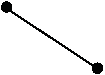
\includegraphics{images/CellConnectionsLine}} &
    \raisebox{-0.5\height}{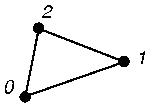
\includegraphics{images/CellConnectionsTriangle}} \\
    \vtkm{CELL\_SHAPE\_VERTEX} &
    \vtkm{CELL\_SHAPE\_LINE} &
    \vtkm{CELL\_SHAPE\_TRIANGLE} \\
    \vtkm{CellShapeTagVertex} \index{vertex} &
    \vtkm{CellShapeTagLine} \index{line} &
    \vtkm{CellShapeTagTriangle} \index{triangle} \\[2ex]
    \raisebox{-0.5\height}{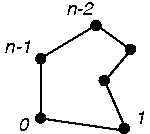
\includegraphics{images/CellConnectionsPolygon}} &
    \raisebox{-0.5\height}{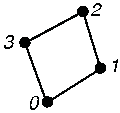
\includegraphics{images/CellConnectionsQuadrilateral}} &
    \raisebox{-0.5\height}{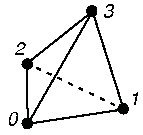
\includegraphics{images/CellConnectionsTetrahedron}} \\
    \vtkm{CELL\_SHAPE\_POLYGON} &
    \vtkm{CELL\_SHAPE\_QUAD} &
    \vtkm{CELL\_SHAPE\_TETRA} \\
    \vtkm{CellShapeTagPolygon} \index{polygon} &
    \vtkm{CellShapeTagQuad} \index{quadrilateral} &
    \vtkm{CellShapeTagTetra} \index{tetrahedron} \\[2ex]
    \raisebox{-0.5\height}{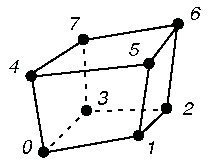
\includegraphics{images/CellConnectionsHexahedron}} &
    \raisebox{-0.5\height}{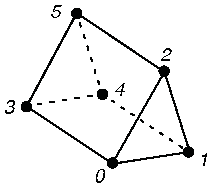
\includegraphics{images/CellConnectionsWedge}} &
    \raisebox{-0.5\height}{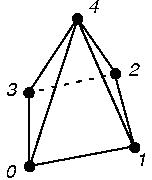
\includegraphics{images/CellConnectionsPyramid}} \\
    \vtkm{CELL\_SHAPE\_HEXAHEDRON} &
    \vtkm{CELL\_SHAPE\_WEDGE} &
    \vtkm{CELL\_SHAPE\_PYRAMID} \\
    \vtkm{CellShapeTagHexahedron} \index{hexahedron} &
    \vtkm{CellShapeTagWedge} \index{wedge} &
    \vtkm{CellShapeTagPyramid} \index{pyramid}
  \end{tabular}
  \caption{Basic Cell Shapes}
  \label{fig:CellShapes}
\end{figure}

In addition to the basic cell shapes, there is a special ``empty'' cell
with the identifier \vtkm{CELL\_SHAPE\_EMPTY} and tag
\vtkm{CellShapeTagEmpty}. This type of cell has no points, edges, or faces
and can be thought of as a placeholder for a null or void cell.

There is also a special cell shape ``tag'' named \vtkm{CellShapeTagGeneric}
that is used when the actual cell shape is not known at compile time.
\textidentifier{CellShapeTagGeneric} actually has a member variable named
\textcode{Id} that stores the identifier for the cell shape. There is no
equivalent identifier for a generic cell; cell shape identifiers can be
placed in a \vtkm{IdComponent} at runtime.

\fix{Add other basic cell shape features such as traits, converting back
  and forth, and \vtkmmacro{vtkmGenericCellShapeMacro}.}

\index{tag!shape|)}
\index{tag!cell~shape|)}
\index{cell~shape|)}
\index{shape|)}

\subsection{Parametric and World Coordinates}

\subsection{Interpolation}

\subsection{Derivatives}
